\chapter{Verification and validation} 
%Last updated 10-03-2016
% Updated 21-10-2016 Got rid of optimisation and added to RKF. Also wrote the TSI part but should still focus on the change in models when writing the complete tool verification and validation including the different test cases.
% Updated 07-11-2016 Small changes to TSI text and wrote the third section on the complete propagation tool.
% Updated 10-11-2016 added sub-section on the validation of the complete tool
% Updated 14-11-2016 continued work on validation section; including the validation cases of Ryan and Joel.
\label{ch:verificationandvalidation}
Verification is the process of determining whether a program meets the requirements or not. Is it working the way it is suppose to? As soon as it works and produces output (verified), these outputs can be compared to other data from which it is known that it is correct. This is called validation. If a program is verified and validated, the outputs should be correct. Fortunately, all the existing software has already been validated, which means that they only still have to be verified to make sure everything is working properly on the simulation computer. Each of the software packages comes with tests which can be used to do this. If all the tests are passed it means that the software is verified for the computer and ready to use. Since \ac{Tudat} shipped with Eigen and Boost, the \ac{Tudat} test files also test these libraries. All the tests were passed, which means that the \ac{Tudat}, Eigen and Boost libraries are working properly. However, because the integrators are an intricate part of this thesis, it was decided to perform a separate verification for the Runge-Kutta integrators. This verification is described in \Cref{sec:rkandrkfver}.

 Mars-\ac{GRAM} also came with its own verification test, where three delivered output files had to be replicated. These verification tests were also successful. 


\section{\acs{RK4} and \acs{RKF} integrators}
\label{sec:rkandrkfver}
The tutorial page of the \ac{Tudat} website \citep{dirkx2016tudat} offers two integration tutorials: one involving \ac{RK4} and another involving variable step-size Runge-Kutta methods including \ac{RKF}. The objective of the tutorial is to get familiar with the different integration methods available in \ac{Tudat}. At the same time, a small data table has to be reproduced, which also serves as a verification test. For each of the integrators the same problem was addressed: the computation of the velocity of a falling body after a certain amount of time assuming no drag. The results that had to be reproduced are presented in \Cref{tab:intverdat}.


\begin{table}[!ht]
\begin{center}
\caption{Verification data for the standard integrators}
\label{tab:intverdat}
\begin{tabular}{|l|l|l|l|l|}
\hline 
\textbf{End time [s]} & 1.0	& 5.0 & 15.0 & 25.0 \\ \hline 
\textbf{Velocity [m/s]} & -9.81 & -49.05 & -147.15 & -245.25 \\ \hline
\end{tabular}
\end{center}
\end{table}

The first script was written using the instructions from the tutorial and is called numericalintegrators.cpp. This script uses the rungeKutta4Integrator.h header file and the RungeKutta4IntegratorXd function from this header file. This function requires three inputs: the state derivative function (problem specific), the initial time and the initial state. Using the .integrateTo extension the end state at a certain end time can be computed. This requires the end time and the step-size. For \ac{RK4} the step-size is constant. This resulted in the same values as presented in \Cref{tab:intverdat}.\\

The second script was used to test the variable step-size integrators \ac{RKF}. This script is called rungekuttavariable.cpp and uses the rungeKuttaCoefficients.h and rungeKuttaVariableStepSizeIntegrator.h header files. In this case the RungeKuttaVariableStepSizeIntegratorXd function was used which requires the Runge-Kutta coefficients (from the respective header file), the state derivative function (problem specific), the initial time, initial state, zero minimum step-size, infinite maximum step-size, relative tolerance and the absolute tolerance as inputs. In this case the integration can be done in individual steps using .performIntegrationStep with the current step-size as the only input. The current step-size is computed in the integration method itself, but in this case it is checked to make sure that the step-size does not take the function beyond the specified end time. The integration steps are then repeated until the end time is met. Running this script resulted in the same results as presented in \Cref{tab:intverdat} as well. \\

These results, combined with the fact that the test files for these two methods produced no errors is proof that they are working accordingly. Thus it can be said that the standard integration methods used in this thesis are verified and ready for use in the simulation tool. However, during the development of the trajectory propagation tools, the entire tool (including the integrators) will be verified again to determine the performance of the integrators.

For the actual propagation tool, the \ac{RKF} method required the state derivative function associated with this particular ascent problem. The state derivative class was constructed using the state derivative functions as described in this thesis in the Cartesian coordinate system based on equations provided by \cite{mooij1994motion}. The state is used to compute the required transformation angles first and then both the thrust and drag accelerations are transformed to the inertial frame. There they are combined with the gravitational acceleration resulting in the accelerations in the x-, y- and z-direction. This class was tested by itself by inputting certain values which would result in known outcomes. And those simple values by themselves provided the expected results. Later the state derivative function was combined with the \ac{RKF} integrator in the trajectory propagation tool and verified again as will be described in \Cref{sec:propverval}. 


The verification of the state derivative class took approximately one day. 



\section{\acl{TSI}}
\label{sec:tsiverval}
In this section, the verification and validation of the \ac{TSI} header and source file is described. This was done for each of the blocks shown in \Cref{fig:TSI_Propagator}. For the verification it was important that the running of the different classes and header/source files did not produce any obvious errors. For the validation, the results were often checked against manual calculations and expected behaviour. The verification and validation of \ac{TSI} was a very lengthy process and required many rewrites of the used equations because of mistakes in the model or mistakes in the derivations. \Cref{sec:propverval} talks a bit more about the model mistakes. This section has been divided into several subsections which showed similar issues during the verification and validation.

\subsection{Auxiliary equations, derivatives and functions}
\label{subsec:auxEqDerFunverval}
As shown by \Cref{fig:TSI_Propagator} the first step in the \ac{TSI} is to compute the auxiliary equations, derivatives and functions. The computations, in theory, are fairly straightforward, however it is really easy to make a mistake. During the initial verification of these different classes the outcomes were checked against simple manual solutions. Thus, provided a certain input, the output was known. This was an easy way to check any coding errors. Since the early versions of the code required a lot of equations, it took a long time to go through all the equations and find all the errors and mistakes. This was initially done with the combination of Cartesian coordinates and spherical transformation angles, however, later on more efficient equations were used for separate Cartesian and spherical cases. This also made it easier to identify mistakes in the equations and understand certain issues found during the validation process. 

\subsection{Computing the Taylor Series coefficients and the updated state}
\label{subsec:TaySerCoefverval}
Once the auxiliary classes were verified, the Taylor Series coefficients could be computed using the basic recurrence relations and the full set of recurrence relations. For the Taylor Series coefficients it is important that they show a decreasing number series for each of the coefficients. This was the desired outcome that was used for the verification of the full set of recurrence relations. The basic recurrence relations were all checked by hand calculations to determine if they indeed worked the way that they were suppose to. The verified basic recurrence relations were used to verify the full set of recurrence relations. This class consists of the equations mentioned in \Cref{app:appendixD-allRecurrenceRelations}. When writing the full set of recurrence relations, it is really easy to make mistakes and there are a lot of rules that have to be taken into account as mentioned in \Cref{ch:tsi}. Therefore, a lot of time was spend on rewriting these equations in such a way that the outcomes were what was expected. Also, a number of these recurrence relations were checked by manual calculations. An often recurring problem was that the Taylor Series coefficients would show a diverging behaviour where the coefficient would keep increasing to infinity (theoretically). This was often an indication that a writing mistake was made when setting up the full set of recurrence relations. Another easy way to identify mistakes during the validation process was to compute the next state. Should an error occur in the computation of the Taylor Series coefficients, this would usually result in very large increases in the state even if the coefficient itself would be relatively small. Then following the trail back to the largest change in Taylor Series coefficient, often a coding or writing mistake could be identified in the full set of recurrence relations. 

\subsection{Next step-size}
\label{subsec:nextStepSizeverval}
Fortunately, the step-size class was not a very large class and took less time to verify and validate. Provided a set of Taylor Series coefficients, the step-size class could be tested separately from the other files. The verification process was rather straight forward; the class should be able to provide a step-size estimate given the different input values. Also, when similar sets of Taylor Series coefficients were used, the output step-sizes should be rather similar. This was then also part of the validation process. A pure validation process was difficult because there were no reference Taylor series coefficients available, however an estimate for the order of the next step-size could be used. This can however still be improved. Two different step-size determination methods were tested, but in the end it was found that the direct method described by \cite{scott2008high} and \cite{bergsma2015application} showed more reasonable results and was easier to implement. Also, during the verification process, the iteration method failed to work properly which led to unusable results and the program failing. But the direct method worked very well.




\section{Complete trajectory propagation}
\label{sec:propverval}
For the complete trajectory propagation it was important to have the integrator method as the only difference between the \ac{RKF} and the \ac{TSI} propagation. First the initial values were provided and transformed into the proper coordinate system. These would then be fed into the integrator and at the end of the integration, the results would be printed. The verification and validation of the complete trajectory propagation have been split up into several phases.


\subsection{Phase 1: \ac{RKF} propagation}
\label{subsec:phase1com}
This was first done for \ac{RKF} because this method was already validated. Therefore, any mistakes or problems found would lead back to a mistake in the state derivative functions or the model itself.
During this phase, a number of problems were identified; certain singularities were found, a limit to the tolerance value was determined for each of the \ac{RKF} methods (\ac{DOPRIN87} does not converge fast enough in many cases for a value of 10$^{-15}$) and a mistake in the model was found where the wrong velocity was used to determine the drag acceleration. This meant that some of the model equations had to be rewritten for both \ac{RKF} and \ac{TSI}. 

\subsection{Phase 2: both \ac{RKF} and \ac{TSI}}
\label{subsec:phase2com}
During the second phase of the verification, both \ac{RKF} and \ac{TSI} were tested at the same time and the outcomes were compared. Since the \ac{RKF} method was verified and validated at this point, the outcome of the \ac{RKF} propagation could be used to verify \ac{TSI}. This was done using different test cases that focussed on different elements of the code. 

Each element was tested separately by activating (or deactivating) the gravity, thrust and drag as well as the rotation of Mars. In each case, simple test cases were used to verify the class, such as: vertical drops from a certain altitude, thrusting in a known direction and flying parabolic trajectories. This was all done in each of the axis directions first and then combining the different axes. First the gravity was tested, then the thrust, then a combination of these two, followed by the drag all in the non-rotating case. The same was then done for the rotating case as well. This was initially done for a zero thrust elevation and thrust azimuth angle, such that the trust was acting directly through the x-axis of the body frame. Also, because the drag by definition works through the x-axis of the body frame, there should not be any accelerations in the y- and z-direction in the body frame. This simplified the problem and meant that some of the equations could be tested without involving all the other equations just yet. 

During this phase it was discovered that there was an inconsistency in the manner in which the different accelerations were computed. Basically, the rotational angles were being computed using spherical equations which already incorporated the accelerations and then those angles were then used to transform the Cartesian coordinates and incorporate the accelerations again. Therefore it was decided to rewrite all the equations and actually come up with three different sets: two Cartesian models and one spherical model for \ac{TSI}. The associated equations were already described in \Cref{ch:tsi}.

\subsection{Phase 3: three different models for \ac{TSI}}
\label{subsec:phase3com}
The third phase consisted of verifying each of these three models in a similar manner as was done during the second phase. During this phase, it was discovered that a starting ground velocity too close to zero would cause singularities in both the Cartesian as well as the spherical model. This is why a small initial ground velocity was introduced, which seemed to work for the second Cartesian case (unit vector transformations) and the spherical case, however, the first Cartesian case (Euler angles) still did not work. At this point it was decided to focus on the other two methods instead because of time constraints. It was also found that the initial flight path angle could not be equal to (or close to) 90 degrees for the spherical case due to singularities in the model. This is why a value of 89 degrees was chosen for the test cases of that particular model. This worked well for gravity and thrust for the spherical and second Cartesian case. But not always.

\subsection{Phase 4: one final \ac{TSI} model}
\label{subsec:phase4com}
As it turned out, setting an initial ground velocity for the \ac{TSI} models (Cartesian and spherical) was only a temporary solution and did not solve the problem. Apparently the initial second is vital for \ac{TSI} and when the velocity is too small, the Taylor Series coefficients tend to increase in value. The solution was to off-set the initial conditions to a later point in the trajectory. This off-set was achieved by having the first second of the trajectory be integrated by \ac{RKF78} with a set tolerance of 10$^{-15}$ (if the method and the tolerance was not set constant, the results of the integration would be inconsistent). When this was applied to the propagation involving \ac{TSI} the Taylor Series coefficients dropped to an acceptable number again which could then be used to determine the next state. This worked really well for the spherical case, however the second Cartesian case still had some bugs (either in the model or in the coding). Again, due to time constraints it was decided to solely continue with the spherical model and use that for the rest of the thesis work. This is the reason that an initial propagation phase was needed as was described in \Cref{sec:completedSimulationTool}. At the end of the phase, the \ac{TSI} code was deemed verified, since it showed similar results to the \ac{RKF} propagation. 

\subsection{Phase 5: coasting and circularisation}
\label{subsec:phase5com}
Once the \ac{TSI} method was verified, the rest of the trajectory propagation could be added. For the coasting phase this meant that the thrust had to be set equal to zero at the point of main engine cut-off. Fortunately, this was a simple change in class value for the \ac{TSI} method, however this did not work for \ac{RKF}. Instead it was discovered that because of the manner in which the state derivative class is set-up and used in the integrator itself, the class had to be re-initialized if anything in the state derivative class changed. Therefore, a new integration had to be started for \ac{RKF} at main engine cut-off. \\

Because the circularisation is treated as an instantaneous burn, this only affected the total propellant mass and velocity of the \ac{MAV}. Therefore, it could be treated with simple circularisation equations described by \cite{wakker2010}. The velocity required to reach a perfect desired circular orbit can be computed. Then because the equations are simple and can be solved by hand, the code could be verified (and validated) by using simple cases computed using the program and then compared to the hand written solutions. 

\subsection{Phase 6: tool validation}
\label{subsec:phase6com}
The most important part of this thesis is the comparison between \ac{RKF} and \ac{TSI}, therefore these two methods should produce results that can be compared and where the only difference is the manner in which they were computed. Provided that the \ac{RKF} method is verified and validated,\ac{TSI} could be validated using \ac{RKF} with this purpose as mentioned before. However, besides this validation, it should also be checked if these solutions represent a real-life solution to the problem. This means validating both methods against other validated simulations outcomes from other people. Unfortunately, no flight data is available for a Mars Ascent case yet. Two \ac{JPL} internal sources were found that could potentially be used to validate the software: \cite{woolley2015simple} and \cite{benito2016trajectory}. Woolley used an analytical model to approximate an ascent trajectory for different launch cases and conditions, one of which was a \ac{SSTO} launcher which was used for validation. Benito on the other hand used a high-fidelity simulation program to simulate the ascent trajectory of some of the newer concept \ac{MAV} designs numerically. Some of the latest data was provided and was also used for the validation.\\

In \Cref{tab:validationCaseWoolley} are the validation numbers provided associated with the simulated trajectory of the case as presented by Woolley. The left columns show the inputs that were provided and the inputs that were used in the program. The right columns show the results of the simulation as provided and as computed by the program. The thrust angles in that column represent the required thrust angles that were needed as input to get the desired outcome.


\begin{table}[!ht]
\begin{center}
\caption{Validation case 1: \ac{SSTO} Woolley}
\label{tab:validationCaseWoolley}
\begin{tabular}{|l|l|l||l||l|l|}
\hline 
\textbf{Provided parameters} & \textbf{Given} & \textbf{Used} & \textbf{Provided parameters} & \textbf{Given} & \textbf{Computed} \\ \hline \hline
Thrust [kN] & 3.56 & 3.56 & Propellant mass [kg] & 202.2 & 202.07 \\ \hline
I$_{sp}$ [s] & 256 & 256 & Burn-out angle [deg] & 6 & 5.344 \\ \hline
Burn Time [s] & 142.6 & 142.5 & Circularisation $\Delta V$ [m/s] & 181 & 159.6 \\ \hline
\ac{MAV} \ac{GLOM} [kg] & 267.4 & 267.4 & Ascent time [s] & 1757 & 1796.27 \\ \hline
Launch altitude [km \ac{MOLA}] & - & -0.6 & Thrust azimuth [deg] & - & -0.299 \\ \hline
Launch latitude [deg] & 0.0 & 0.0 & Thrust elevation [deg] & - & -0.184 \\ \hline
Launch longitude [deg] & - & 74.5 & & & \\ \hline
Launch ground velocity [km/s] & - & 1$\cdot $ 10$^{-5}$ & & & \\ \hline
Launch \ac{FPA} [deg] & 90 & 89 & & & \\ \hline
Launch Azimuth [deg] & 90 & 90 & & & \\ \hline
Desired altitude [km \ac{MOLA}] & 390 & 390 & & & \\ \hline
Desired inclination [deg] & 45 & 45 & & & \\ \hline




\end{tabular}
\end{center}
\end{table}

It can be seen that there are some differences, however in this case the validation is to prove that the trajectory computed by the simulation program is indeed a viable trajectory (so close to a reference trajectory). This is because that is enough to compare the \ac{RKF} and \ac{TSI} methods. The plotted trajectories are shown in \Cref{fig:PlotFigure2Zoom,fig:PlotFigure1SeenFromZoomXaxis,fig:PlotFigure1SeenFromZoomYaxis,fig:PlotFigure1SeenFromZoomZaxis}.

\begin{figure}[!ht]
\centering
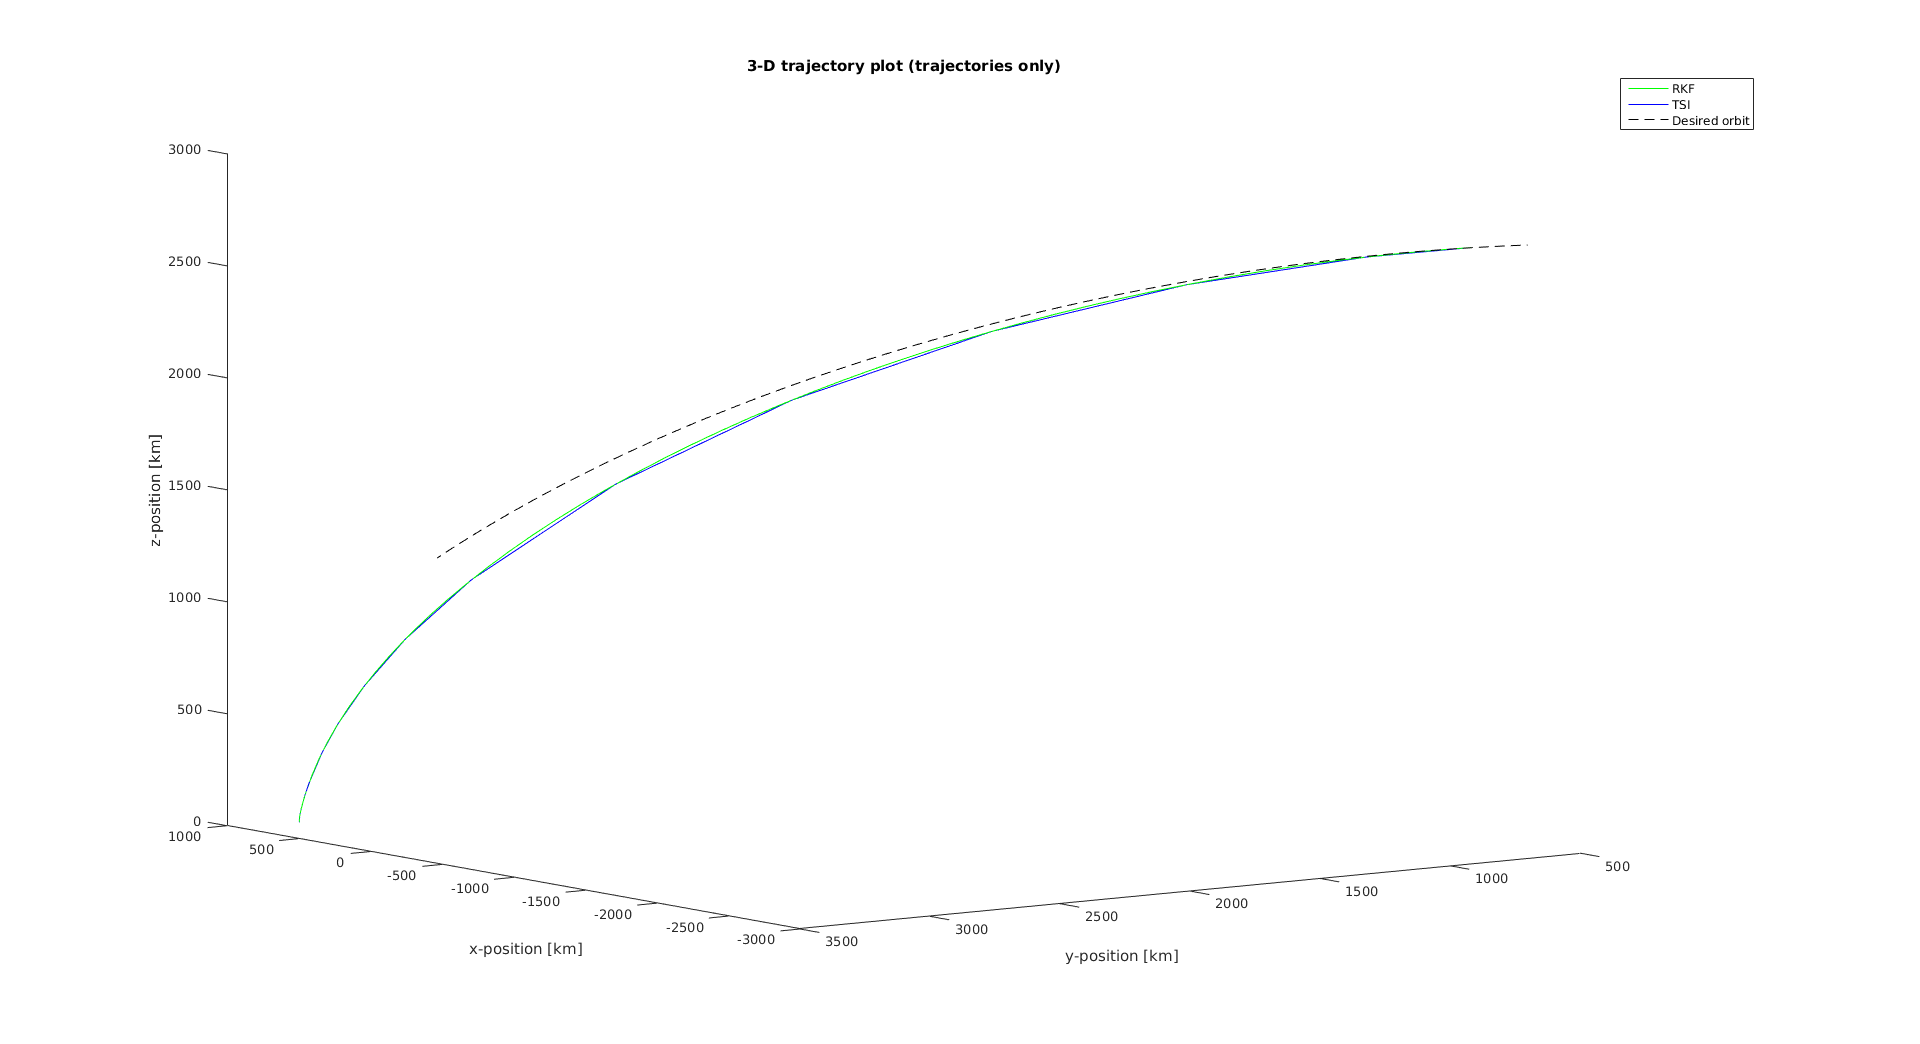
\includegraphics[width=0.8 \textwidth]{figures/verification/case1/PlotFigure2Zoom.png}
\caption{Case 1 3-D trajectory}
\label{fig:PlotFigure2Zoom}
\end{figure}

\begin{figure}[!ht]
\centering
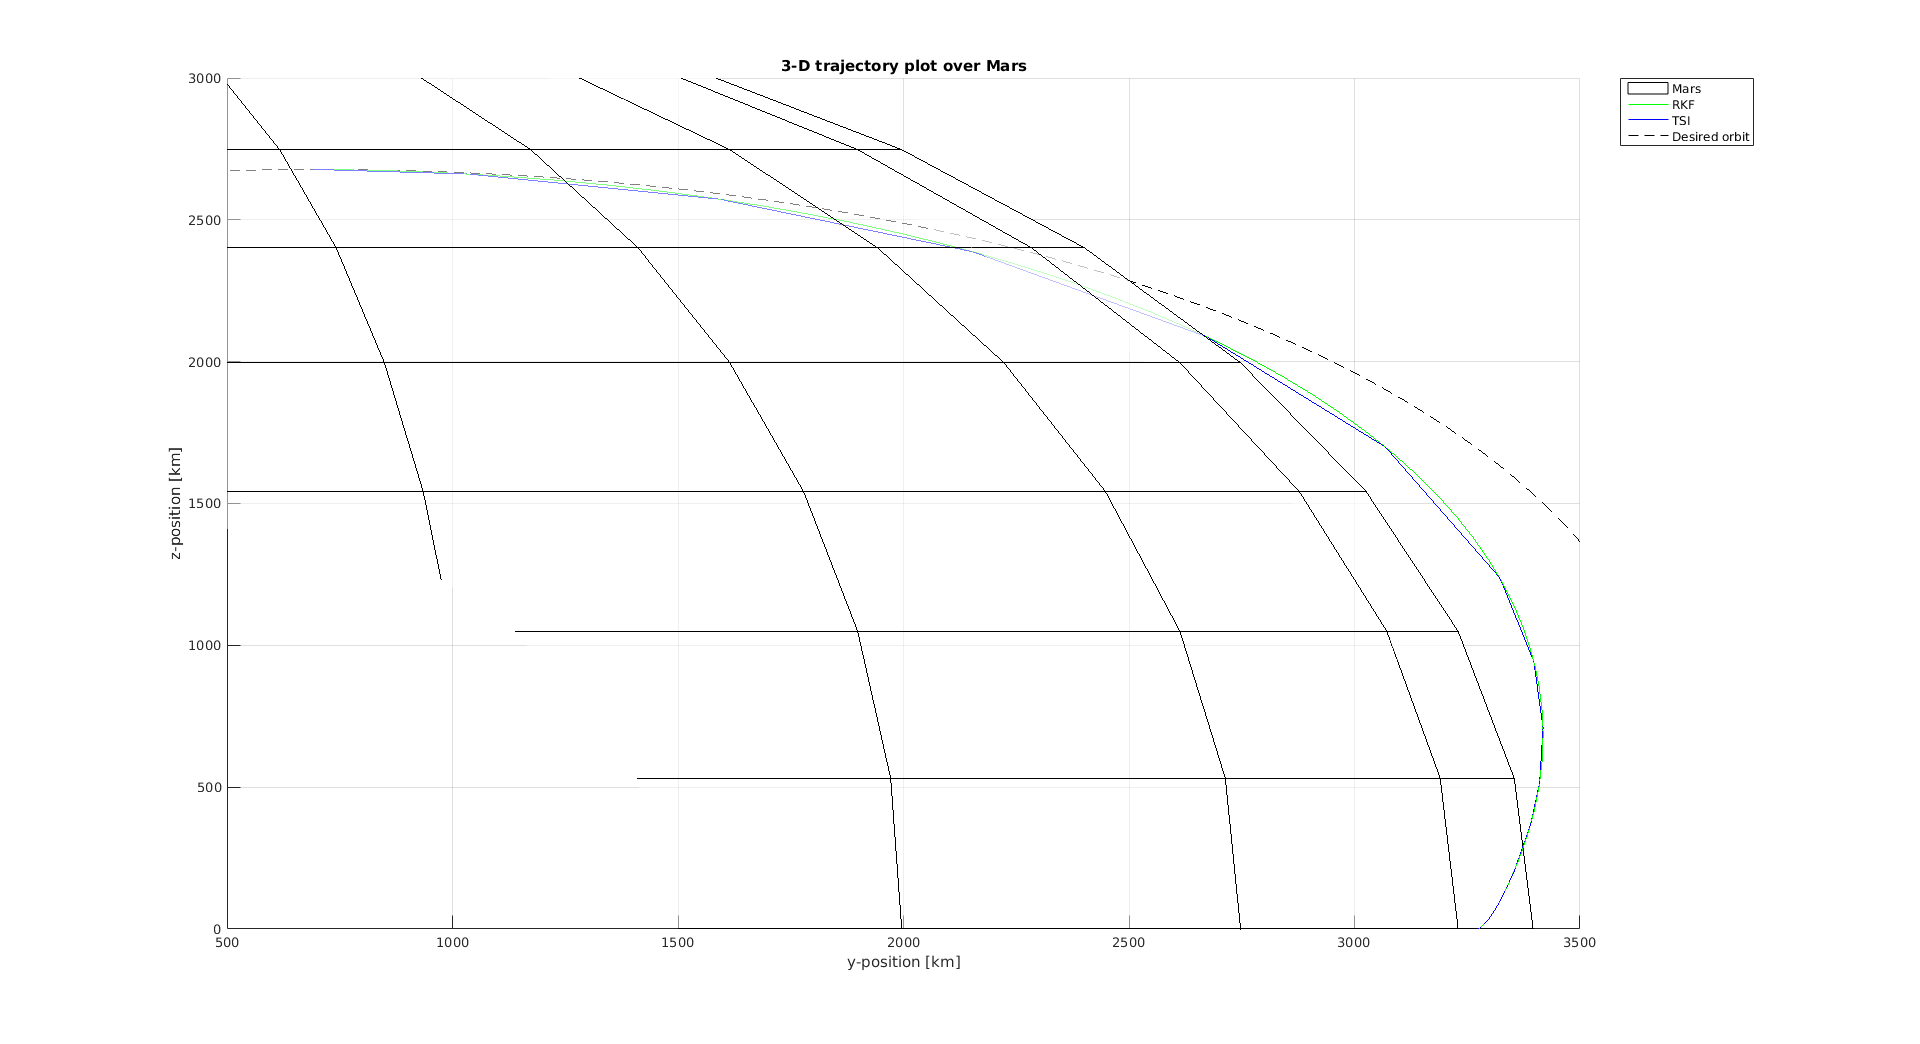
\includegraphics[width=0.8 \textwidth]{figures/verification/case1/PlotFigure1SeenFromZoomXaxis.png}
\caption{Case 1 2-D trajectory as seen from the x-axis}
\label{fig:PlotFigure1SeenFromZoomXaxis}
\end{figure}

\begin{figure}[!ht]
\centering
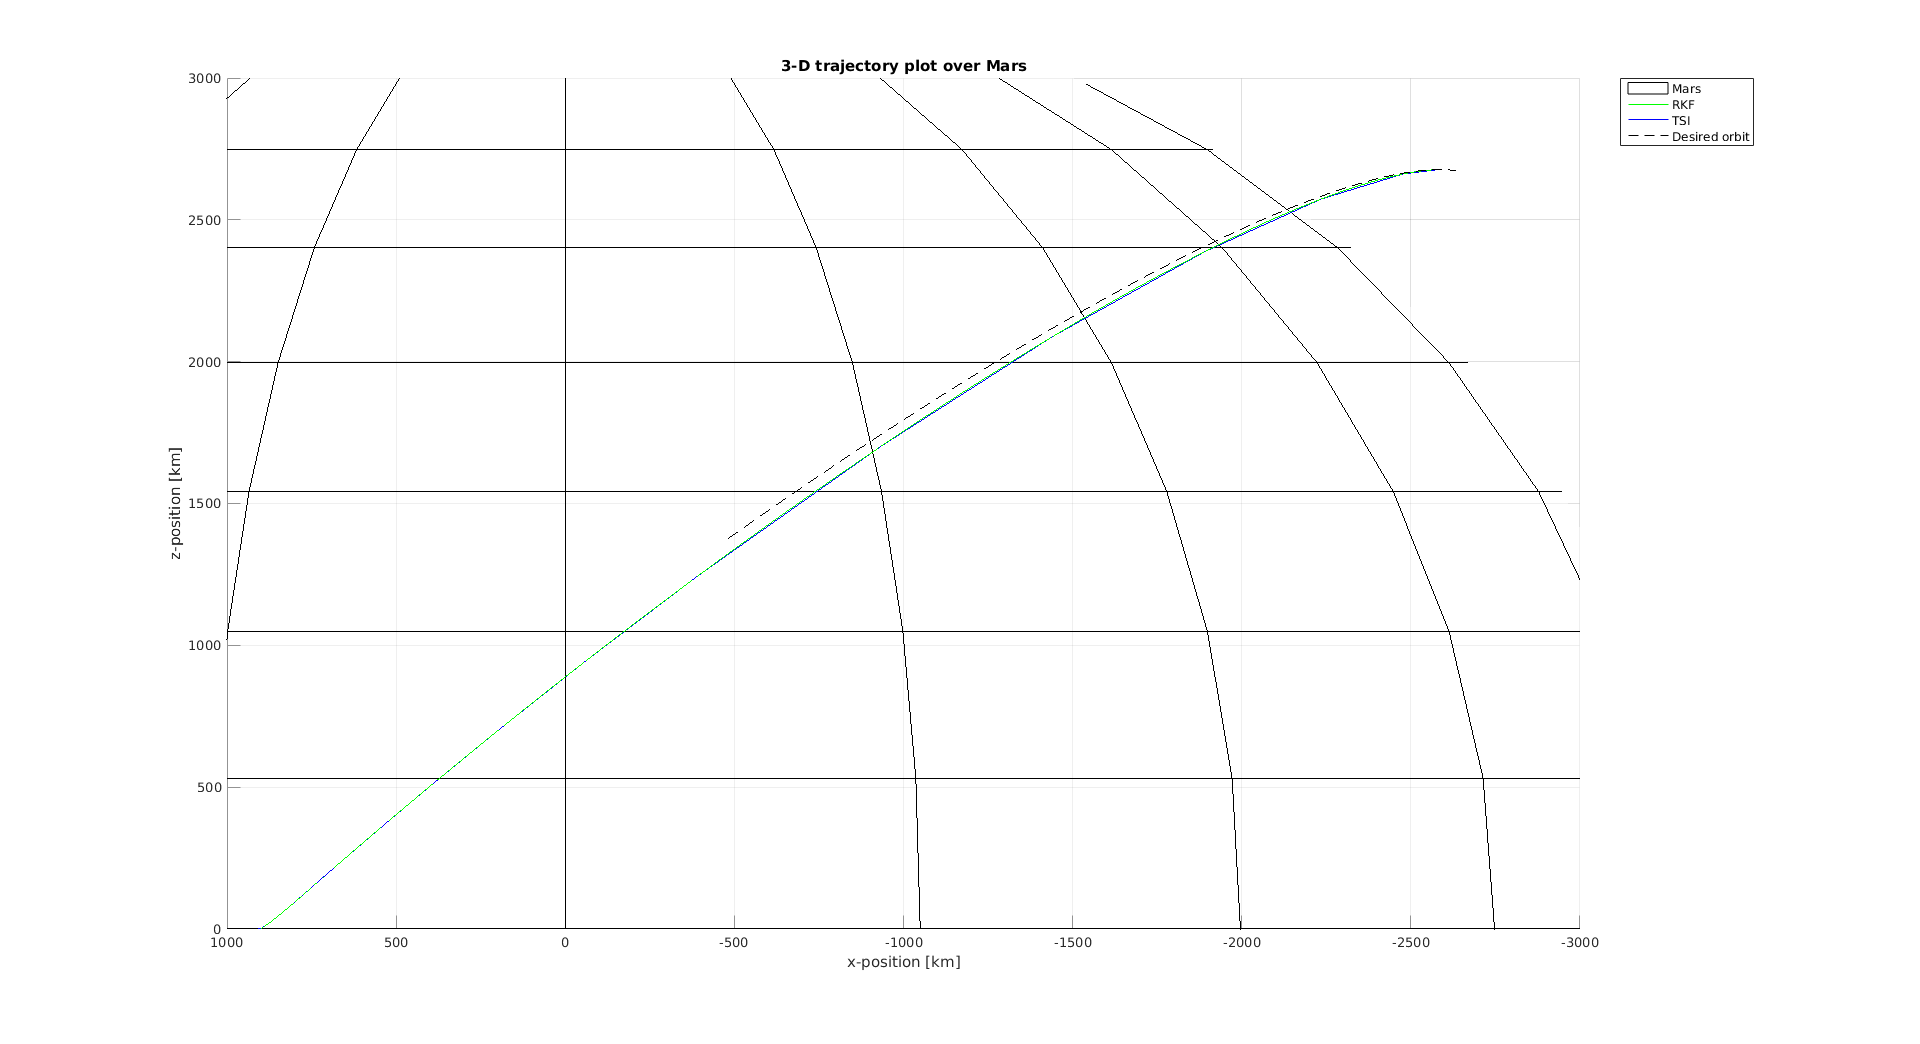
\includegraphics[width=0.8 \textwidth]{figures/verification/case1/PlotFigure1SeenFromZoomYaxis.png}
\caption{Case 1 2-D trajectory as seen from the y-axis}
\label{fig:PlotFigure1SeenFromZoomYaxis}
\end{figure}

\begin{figure}[!ht]
\centering
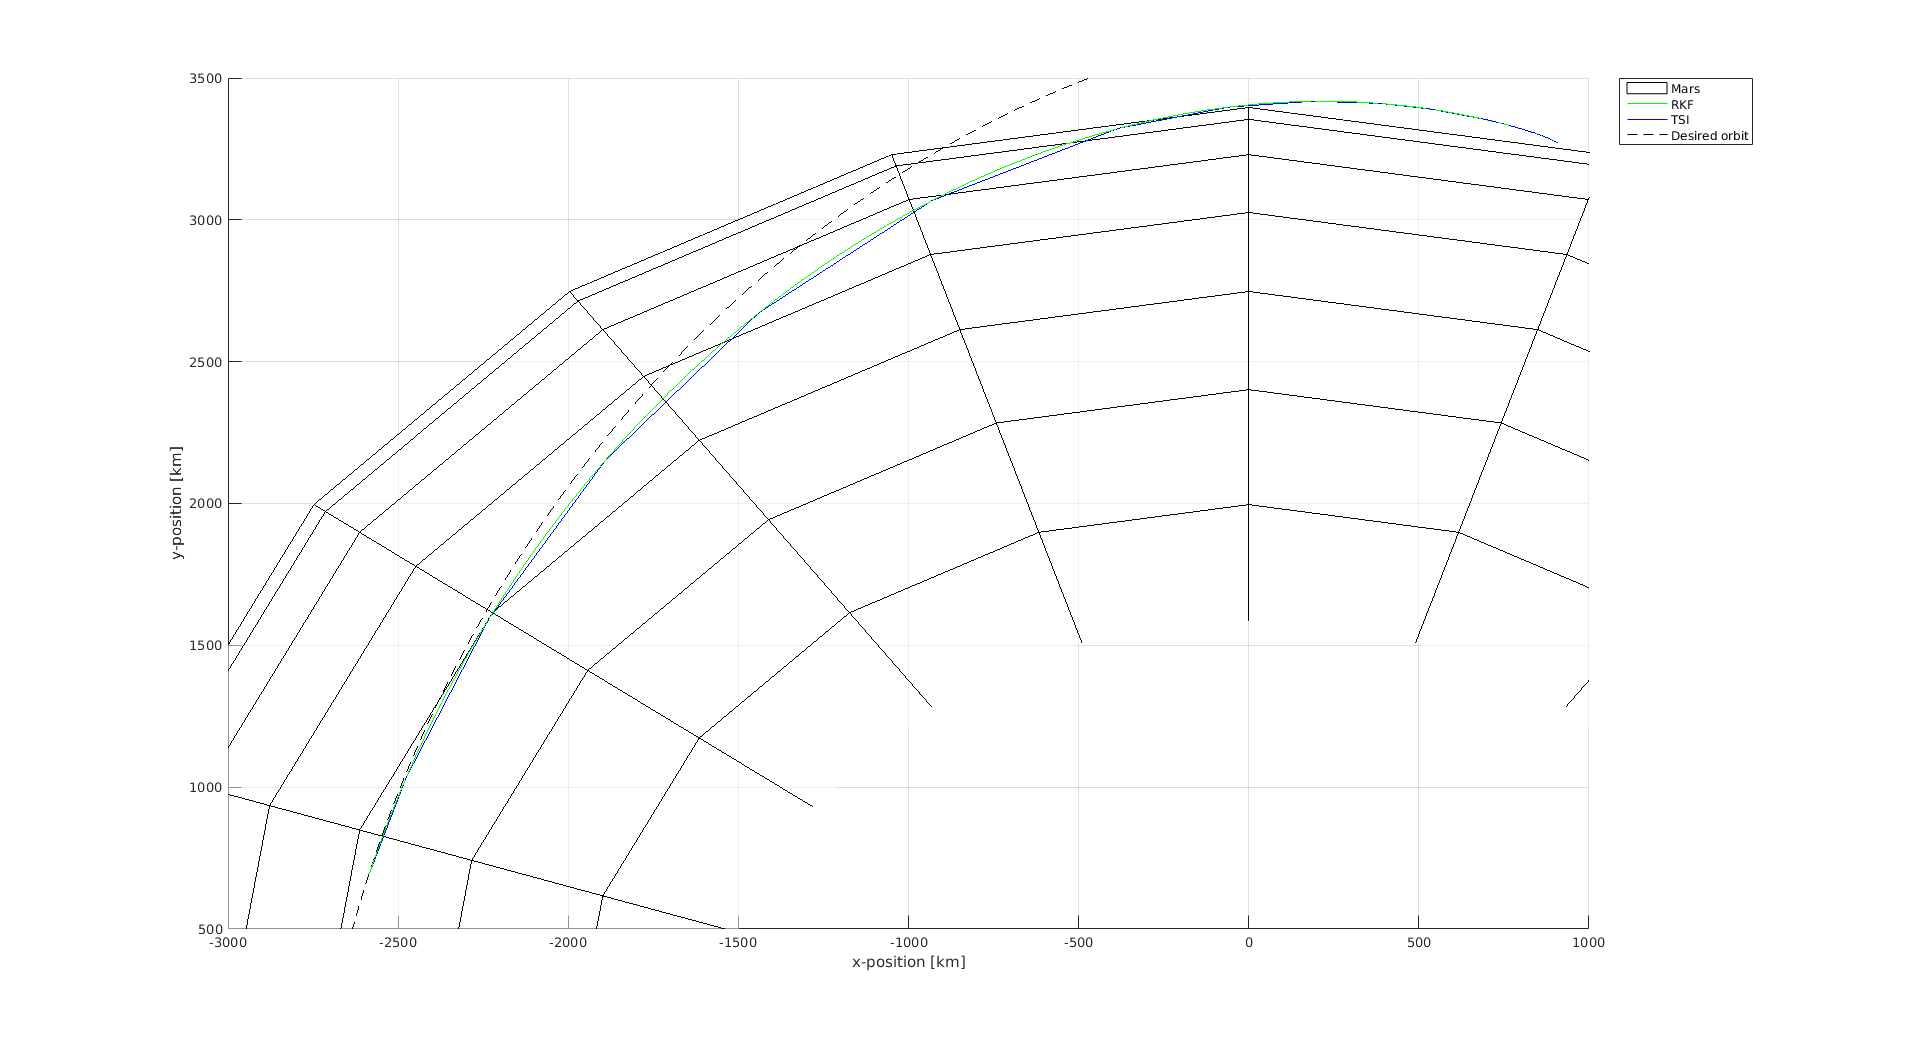
\includegraphics[width=0.8 \textwidth]{figures/verification/case1/PlotFigure1SeenFromZoomZaxis.png}
\caption{Case 1 2-D trajectory as seen from the z-axis}
\label{fig:PlotFigure1SeenFromZoomZaxis}
\end{figure}

A similar validation was done using the second case. However, in this case the reference trajectory was provided. But the main difference here was that the simulation program still was only able to use a constant thrust elevation and azimuth angle. Therefore, the exact profile could not be matched. Benito also included extra perturbing effects creating another difference.  




\begin{table}[!ht]
\begin{center}
\caption{Validation case 2: \ac{SSTO} Benito}
\label{tab:validationCaseBenito}
\begin{tabular}{|l|l|l||l||l|l|}
\hline 
\textbf{Provided parameters} & \textbf{Given} & \textbf{Used} & \textbf{Provided parameters} & \textbf{Given} & \textbf{Computed} \\ \hline \hline
Thrust [kN] & 6.1087 & 6.0187 & Propellant mass [kg] & 213.85 & 213.85 \\ \hline
I$_{sp}$ [s] & 315.9 & 315.9 & Burn-out angle [deg] & - & 15.644 \\ \hline
Burn Time [s] & 99.362 & 99.362 & Circularisation $\Delta V$ [m/s] & 757.57 & 594.74 \\ \hline
\ac{MAV} \ac{GLOM} [kg] & 288.96 & 288.96 & Ascent time [s] & 949.12 & 876.09 \\ \hline
Launch altitude [km \ac{MOLA}] & -0.8 & -0.6 & Thrust azimuth [deg] & - & -0.7273 \\ \hline
Launch latitude [deg] & 0.0 & 0.0 & Thrust elevation [deg] & - & -0.674 \\ \hline
Launch longitude [deg] & 90 & 90 & & & \\ \hline
Launch ground velocity [km/s] & 1$\cdot $ 10$^{-6}$ & 1$\cdot $ 10$^{-6}$ & & & \\ \hline
Launch \ac{FPA} [deg] & 90 & 89 & & & \\ \hline
Launch Azimuth [deg] & 90 & 90 & & & \\ \hline
Desired altitude [km \ac{MOLA}] & 479.19 & 479.19 & & & \\ \hline
Desired inclination [deg] & 92.69 & 92.69 & & & \\ \hline




\end{tabular}
\end{center}
\end{table}

%\section{Optimiser}
%\label{sec:optver}
%
%
%\section{Complete optimisation tool}
%\label{sec:opttoolverval}


